% =============================================================================
% PRESENTACIÓN CANDIDATURA DOCTORAL
% Sistema Híbrido para Predicción de Emisiones de CO₂ y CH₄
% en la Bioconversión de Residuos con Hermetia illucens
% =============================================================================
% Compilación: make candidatura (o xelatex -> latexmk)
% =============================================================================

\documentclass[aspectratio=169, 11pt]{beamer}

% =============================================================================
% 1. PREÁMBULO: FUENTES Y PAQUETES (XELATEX)
% =============================================================================
\usepackage{fontspec}
\setmainfont{TeX Gyre Termes}
\setsansfont{TeX Gyre Heros}
\setmonofont{Latin Modern Mono}

\usepackage[spanish,es-nodecimaldot]{babel}
\usepackage{amsmath, amssymb, amsfonts}
\usepackage{booktabs}
\usepackage{array}
\usepackage{graphicx}
\usepackage{tikz}

% Librerías TikZ
\usetikzlibrary{shapes.geometric, arrows.meta, positioning, calc, fit, shadows, shapes.symbols, backgrounds}

% =============================================================================
% 2. TEMA Y COLORES
% =============================================================================
\usetheme{Madrid}
\usecolortheme{beaver}

% Colores personalizados (UNAL-inspired)
\definecolor{unalRojo}{RGB}{148, 36, 36}
\definecolor{unalGris}{RGB}{80, 80, 80}
\definecolor{verdeOK}{RGB}{34, 139, 34}
\definecolor{naranjaAlerta}{RGB}{230, 126, 34}
\definecolor{rojoAlerta}{RGB}{192, 57, 43}

\setbeamercolor{structure}{fg=unalRojo}
\setbeamercolor{block title}{bg=unalRojo!15, fg=unalRojo}
\setbeamercolor{block body}{bg=unalRojo!5}
\setbeamercolor{alerted text}{fg=rojoAlerta}

% =============================================================================
% 3. METADATOS
% =============================================================================
\title[Sistema Híbrido BSF]{Sistema Híbrido para Predicción de Emisiones de CO$_2$ y CH$_4$}
\subtitle{en la Bioconversión de Residuos con \textit{Hermetia illucens}}
\author{John Jairo Leal Gómez}
\institute[UNAL]{Doctorado en Estudios Ambientales\\Universidad Nacional de Colombia -- Sede Palmira}
\date{Abril 2026}
\titlegraphic{
\includegraphics[width=1.8cm]{../tesis/00Figuras/00f00EscudoUN2016.jpg}}

% =============================================================================
% 4. COMANDOS PERSONALIZADOS
% =============================================================================
\newcommand{\BSF}{\textit{Hermetia illucens}}
\newcommand{\COtwo}{CO$_2$}
\newcommand{\CHfour}{CH$_4$}
\newcommand{\MAPE}{\text{MAPE}}
\newcommand{\DEB}{\text{DEB}}
\newcommand{\NDIR}{\text{NDIR}}
\newcommand{\MRV}{\text{MRV}}

% =============================================================================
% 5. CONFIGURACIÓN DE BEAMER
% =============================================================================
\setbeamertemplate{navigation symbols}{}
\setbeamertemplate{footline}[frame number]
\setbeamertemplate{caption}[numbered]

% =============================================================================
% INICIO DEL DOCUMENTO
% =============================================================================
\begin{document}

% =============================================================================
% SLIDE 1: PORTADA
% =============================================================================
\begin{frame}[plain]
    \titlepage
\end{frame}

% =============================================================================
% SLIDE 2: ÍNDICE
% =============================================================================
\begin{frame}{Índice de la Presentación}
    \tableofcontents
\end{frame}

% =============================================================================
% SECCIÓN 1: EL PROBLEMA CLIMÁTICO (5 min)
% =============================================================================
\section{El Problema Climático}

\begin{frame}{Concentraciones Récord de GEI en 2024}
    \begin{columns}[T]
        \column{0.55\textwidth}
        \begin{alertblock}{Datos WMO 2025}
            \begin{itemize}
                \item \textbf{CO$_2$:} 423.9 ppm (nivel sin precedentes)
                \item \textbf{CH$_4$:} 1942 ppb (potencial de calentamiento 28$\times$ CO$_2$)
                \item \textbf{N$_2$O:} 338.0 ppb
            \end{itemize}
        \end{alertblock}

        \vspace{0.3cm}
        \textbf{La paradoja del 0.042\%:}\\
        \small No es abundancia relativa, sino \textbf{propiedades radiativas intrínsecas} de la molécula. El forzamiento radiativo se ha alterado irreversiblemente.

        \column{0.45\textwidth}
        \centering
        \begin{tikzpicture}[scale=0.8]
            % Barras verticales simuladas
            \fill[unalRojo!30] (0,0) rectangle (1,4.239);
            \fill[naranjaAlerta!50] (1.5,0) rectangle (2.5,1.942);
            \fill[verdeOK!40] (3,0) rectangle (4,1.5);

            \node[below, font=\tiny] at (0.5,0) {CO$_2$};
            \node[below, font=\tiny] at (2,0) {CH$_4$};
            \node[below, font=\tiny] at (3.5,0) {N$_2$O};

            \node[above, font=\tiny, rotate=90] at (0.5,2) {423.9 ppm};
            \node[above, font=\tiny, rotate=90] at (2,0.9) {1942 ppb};

            \draw[->, thick] (-0.5,0) -- (4.5,0) node[right, font=\tiny] {Concentración};
            \draw[->, thick] (-0.5,0) -- (-0.5,5) node[above, font=\tiny] {Nivel};
        \end{tikzpicture}

        \vspace{0.3cm}
        \footnotesize \textit{Fuente: WMO Greenhouse Gas Bulletin No. 21}
    \end{columns}
\end{frame}

\begin{frame}{Gestión de Residuos: Fuente Crítica de CH$_4$}
    \begin{columns}[T]
        \column{0.5\textwidth}
        \begin{block}{La realidad del Sur Global}
            \begin{itemize}
                \item $>$50\% de residuos sólidos son orgánicos
                \item Dispersión geográfica y estacionalidad
                \item Infraestructura de tratamiento limitada
            \end{itemize}
        \end{block}

        \vspace{0.3cm}
        \textbf{Descomposición anaerobia} en rellenos sanitarios:\\
        \small Generación de CH$_4$ durante años/décadas, prácticamente incontrolable.

        \column{0.5\textwidth}
        \begin{alertblock}{Soluciones convencionales: ¿Viables?}
            \begin{itemize}
                \item \textbf{Rellenos sanitarios:} Emisiones prolongadas, difusas
                \item \textbf{Digestión anaerobia:} Infraestructura compleja, costosa
                \item \textbf{Compostaje:} N$_2$O + tiempos largos de estabilización
            \end{itemize}
        \end{alertblock}

        \vspace{0.3cm}
        \centering
        \footnotesize \textit{En el Valle del Cauca, estas alternativas son técnicamente o económicamente inviables a escala agroindustrial.}
    \end{columns}
\end{frame}

% =============================================================================
% SECCIÓN 2: BSF COMO ALTERNATIVA (6 min)
% =============================================================================
\section{Bioconversión con \textit{Hermetia illucens}}

\begin{frame}{\BSF{}: De Residuo a Recurso en 3--4 Semanas}
    \begin{columns}[T]
        \column{0.5\textwidth}
        \begin{block}{Proceso de economía circular}
            \begin{itemize}
                \item \textbf{Entrada:} Residuos orgánicos agroindustriales
                \item \textbf{Proceso:} Larvas en estadios voraces (L3--L5)
                \item \textbf{Salidas:}
                \begin{itemize}
                    \item Biomasa rica en proteínas y lípidos
                    \item Frass (fertilizante orgánico)
                \end{itemize}
            \end{itemize}
        \end{block}

        \vspace{0.2cm}
        \textbf{Reducción de masa:} 50--80\% (base húmeda)\\
        \textbf{Incremento larval:} Hasta 4000$\times$ su masa inicial

        \column{0.5\textwidth}
        \centering
        \begin{tikzpicture}[scale=0.75, transform shape,
            caja/.style={rectangle, rounded corners, draw, minimum width=2.5cm, minimum height=1cm, align=center, font=\small}]

            \node[caja, fill=green!15] (res) at (0,3) {Residuos\\Orgánicos};
            \node[caja, fill=orange!15] (lar) at (0,1.5) {Larvas \BSF\\(Metabolismo)};
            \node[caja, fill=blue!15] (bio) at (-2,0) {Biomasa\\(Proteína)};
            \node[caja, fill=brown!20] (fra) at (2,0) {Frass\\(Fertilizante)};

            \draw[->, thick] (res) -- (lar);
            \draw[->, thick] (lar) -- (bio);
            \draw[->, thick] (lar) -- (fra);

            \node[right=0.3cm of lar, font=\tiny, text width=2cm] {CO$_2$ + Calor\\(Metabolismo)};
        \end{tikzpicture}

        \vspace{0.3cm}
        \footnotesize \textit{Ventajas clave: menor infraestructura, sin lixiviados, tiempos cortos, operable a pequeña escala.}
    \end{columns}
\end{frame}

\begin{frame}{El Problema de la ``Caja Negra''}
    \begin{columns}[T]
        \column{0.55\textwidth}
        \begin{alertblock}{Vacío crítico de información}
            \begin{itemize}
                \item Se conocen \textbf{entradas} (residuos) y \textbf{salidas} (biomasa, frass)
                \item Se desconocen los \textbf{flujos gaseosos intermedios}
                \item No existen \textbf{factores de emisión específicos} para BSF en IPCC ni GHG Protocol
            \end{itemize}
        \end{alertblock}

        \vspace{0.2cm}
        \textbf{Consecuencia:} Cualquier balance de carbono se basa en supuestos no verificados.

        \vspace{0.2cm}
        \begin{exampleblock}{Riesgo de greenwashing}
            Sin monitoreo riguroso, BSF podría emitir \textbf{más CH$_4$ que el compostaje} en condiciones de anaerobiosis no controlada.
        \end{exampleblock}

        \column{0.45\textwidth}
        \centering
        \begin{tikzpicture}[scale=0.7, transform shape]
            \node[draw, dashed, rounded corners, fill=gray!10, minimum width=3cm, minimum height=3cm, align=center] (caja) at (0,0) {\textbf{?}\\[0.2cm]\footnotesize Dinámica de\\[-0.1cm]emisiones\\[-0.1cm]desconocida};

            \node[fill=green!20, rounded corners, minimum width=1.5cm, minimum height=0.8cm, font=\small] (in) at (-3,0) {Residuos};
            \node[fill=blue!20, rounded corners, minimum width=1.5cm, minimum height=0.8cm, font=\small] (out1) at (3,1) {Biomasa};
            \node[fill=brown!20, rounded corners, minimum width=1.5cm, minimum height=0.8cm, font=\small] (out2) at (3,-1) {Frass};

            \draw[->, thick] (in) -- (caja);
            \draw[->, thick] (caja) -- (out1);
            \draw[->, thick] (caja) -- (out2);

            \node[font=\tiny, text=red!70!black] at (0,-2) {CH$_4$ fugitivo?};
        \end{tikzpicture}
    \end{columns}
\end{frame}

% =============================================================================
% SECCIÓN 3: SISTEMA HÍBRIDO (14 min) - NÚCLEO
% =============================================================================
\section{La Propuesta: Sistema Híbrido}

\begin{frame}{¿Por qué un Sistema Híbrido?}
    \begin{block}{La convergencia estructural de tres componentes}
        Ninguno por sí solo puede validar la sostenibilidad ambiental del proceso. Solo su \textbf{integración} transforma datos crudos en evidencia verificable.
    \end{block}

    \vspace{0.3cm}
    \centering
    \begin{tikzpicture}[scale=0.9, transform shape,
        comp/.style={rectangle, rounded corners, draw, minimum width=3.5cm, minimum height=1.2cm, align=center, font=\small\bfseries},
        flecha/.style={->, thick, >=stealth}]

        % Componentes
        \node[comp, fill=gray!15] (sens) at (0,2.5) {Sensores IoT\\(NDIR CO$_2$/CH$_4$)};
        \node[comp, fill=blue!10] (edo) at (-3.5,0) {Modelo Matemático\\(EDO / \DEB)};
        \node[comp, fill=orange!10] (ia) at (3.5,0) {Aprendizaje Automático\\(RNA / PINNs)};

        % Triángulo de integración
        \node[comp, fill=unalRojo!15, draw=unalRojo, line width=1.5pt] (hibr) at (0,-2.5) {SISTEMA HÍBRIDO\\Predicción + Alertas};

        % Flechas
        \draw[flecha] (sens) -- (edo);
        \draw[flecha] (sens) -- (ia);
        \draw[flecha] (edo) -- (hibr);
        \draw[flecha] (ia) -- (hibr);
        \draw[flecha, dashed] (edo) -- node[above, font=\tiny] {Corrección} (ia);

        % Etiquetas de limitación
        \node[below=0.1cm of sens, font=\tiny, text=gray] {``Ceguera semántica''};
        \node[left=0.1cm of edo, font=\tiny, text=gray, align=right] {``Rigidez''\\ ante variabilidad};
        \node[right=0.1cm of ia, font=\tiny, text=gray, align=left] {``Opacidad''\\ caja negra};
    \end{tikzpicture}
\end{frame}

\begin{frame}{Arquitectura en Cascada: De Sensor a Decisión}
    \begin{columns}[T]
        \column{0.55\textwidth}
        \textbf{Etapa 1 -- Inferencia Biométrica (RNA):}
        \begin{itemize}
            \item Entradas: temperatura, humedad, histórico de emisiones
            \item Salida: biomasa húmeda $W(t)$ y estadio larval \textit{en tiempo real}
            \item \textit{Problema resuelto:} medición directa es invasiva
        \end{itemize}

        \vspace{0.2cm}
        \textbf{Etapa 2 -- Modelado Metabólico (\DEB):}
        \begin{itemize}
            \item Desagregación del flujo energético
            \item CO$_2$ = mantenimiento somático + síntesis de tejido
            \item Supuesto: aerobiosis estricta
        \end{itemize}

        \vspace{0.2cm}
        \textbf{Etapa 3 -- Diagnóstico por Contrastación:}
        \begin{itemize}
            \item $Y_{sensor} = Y_{modelo} + \delta_{bio} + \epsilon_{inst}$
            \item Divergencia + CH$_4$ detectado $\Rightarrow$ \textbf{anaerobiosis}
        \end{itemize}

        \column{0.45\textwidth}
        \centering
        \begin{tikzpicture}[scale=0.65, transform shape,
            etapa/.style={rectangle, rounded corners, draw, minimum width=2.8cm, minimum height=1cm, align=center, font=\small}]

            \node[etapa, fill=orange!15] (rna) at (0,3) {RNA\\$W(t)$};
            \node[etapa, fill=blue!10] (deb) at (0,1.5) {Modelo \DEB\\$Y_{CO_2}$ teórico};
            \node[etapa, fill=red!10] (diag) at (0,0) {Diagnóstico\\Alerta};

            \node[left=0.5cm of rna, font=\tiny, align=right] {T, HR,\\CO$_2$ hist.};
            \node[right=0.5cm of diag, font=\tiny, align=left] {Semaforización\\Verde/Ambar/Rojo};

            \draw[->, thick] (rna) -- (deb);
            \draw[->, thick] (deb) -- (diag);
            \draw[->, thick, dashed] (rna.west) to[bend left=30] node[left, font=\tiny] {Real} (diag.west);
        \end{tikzpicture}

        \vspace{0.3cm}
        \footnotesize \textit{La ``inteligencia'' reside en la integración, no en ningún componente aislado.}
    \end{columns}
\end{frame}

\begin{frame}{Flujo Metabólico DEB: De Dónde Sale el CO$_2$}
    \begin{columns}[T]
        \column{0.4\textwidth}
        \begin{block}{Lógica del carbono}
            El alimento entra al pool de \textbf{Asimilados ($A$)} y se distribuye. El CO$_2$ se genera como ``costo'' en tres puntos:
        \end{block}
        \small
        \begin{enumerate}
            \item \textbf{$r_{CO2,m}$:} Mantenimiento (costo fijo de vivir)
            \item \textbf{$r_{CO2,B}$:} Estructura (costo de crecer)
            \item \textbf{$r_{CO2,L}$:} Lípidos (costo de reservas)
        \end{enumerate}

        \vspace{0.2cm}
        \centering
        \large
        $r_{CO2} = r_{CO2,m} + r_{CO2,B} + r_{CO2,L}$

        \column{0.6\textwidth}
        \centering
        \begin{tikzpicture}[scale=0.8, transform shape,
            caja/.style={rectangle, draw, thick, rounded corners, fill=white, align=center, font=\footnotesize\bfseries, minimum height=0.9cm, drop shadow},
            gas/.style={rectangle, draw, dashed, thick, fill=gray!5, minimum width=3.5cm, minimum height=0.7cm, font=\small}]

            \draw[fill=gray!10, draw=none, rounded corners=12pt] (-3.2, -1.3) rectangle (3.2, 1.3);
            \node[gray!50, font=\tiny, anchor=south] at (0,-1.3) {Larva};

            \node[caja, text width=1.8cm] (A) at (0, 0) {Asimilados\\$A$};
            \node[caja, text width=1.8cm] (B) at (-2.8, 0) {Estructura\\$B$};
            \node[caja, text width=1.8cm] (L) at (2.8, 0) {Lípidos\\$L$};
            \node[gas] (CO2) at (0, 2.2) {\large CO$_2$};

            \draw[->, thick, >=stealth] (0, -1.3) -- node[fill=white, inner sep=1pt, font=\tiny] {$r_A$} (A);
            \draw[->, thick, >=stealth] (A) -- node[below, font=\tiny] {$r_B$} (B);
            \draw[->, thick, >=stealth] ([yshift=1.5mm]A.east) -- node[above, font=\tiny] {$r_L$} ([yshift=1.5mm]L.west);
            \draw[->, thick, >=stealth, dashed] ([yshift=-1.5mm]L.west) -- ([yshift=-1.5mm]A.east);

            \draw[->, thick, >=stealth] (A.north) -- node[fill=white, inner sep=1pt, font=\tiny] {$r_{CO2,m}$} (CO2.south);
            \draw[->, thick, >=stealth] (-1.4, 0.2) -- (-1.4, 1.8) node[midway, fill=white, inner sep=1pt, font=\tiny] {$r_{CO2,B}$};
            \draw[->, thick, >=stealth] (1.4, 0.2) -- (1.4, 1.8) node[midway, fill=white, inner sep=1pt, font=\tiny] {$r_{CO2,L}$};
        \end{tikzpicture}
    \end{columns}
\end{frame}

\begin{frame}{Arquitectura Tecnológica de 3 Capas}
    \centering
    \begin{tikzpicture}[scale=0.85, transform shape,
        capa/.style={rectangle, rounded corners, draw, minimum width=11cm, minimum height=1.6cm, align=left, font=\small},
        comp/.style={rectangle, rounded corners, fill=white, draw, minimum width=2.2cm, minimum height=0.9cm, align=center, font=\tiny}]

        % Capa 1: Percepción
        \node[capa, fill=green!8] (per) at (0,3) {};
        \node[font=\bfseries\small, anchor=north west] at (-5,3.6) {1. Percepción (Edge)};
        \node[comp, fill=green!15] at (-3.5,3) {ESP32};
        \node[comp, fill=green!15] at (-1,3) {NDIR CO$_2$};
        \node[comp, fill=green!15] at (1.5,3) {NDIR CH$_4$};
        \node[comp, fill=green!15] at (4,3) {T/HR};

        % Capa 2: Procesamiento
        \node[capa, fill=blue!8] (pro) at (0,1) {};
        \node[font=\bfseries\small, anchor=north west] at (-5,1.6) {2. Procesamiento (Core)};
        \node[comp, fill=blue!15] at (-3,1) {PostgreSQL};
        \node[comp, fill=blue!15] at (0,1) {Motor \DEB};
        \node[comp, fill=orange!15] at (3,1) {Corrección RNA};

        % Capa 3: Aplicación
        \node[capa, fill=red!8] (app) at (0,-1) {};
        \node[font=\bfseries\small, anchor=north west] at (-5,-0.4) {3. Aplicación (Dashboard)};
        \node[comp, fill=red!15] at (-3,-1) {Next.js};
        \node[comp, fill=red!15] at (0,-1) {Semaforización};
        \node[comp, fill=red!15] at (3,-1) {Reporte MRV};

        % Conexiones
        \draw[->, thick, >=stealth] (per) -- (pro);
        \draw[->, thick, >=stealth] (pro) -- (app);

        % Protocolos
        \node[font=\tiny, text=gray] at (0,2.1) {MQTT / LoRaWAN};
        \node[font=\tiny, text=gray] at (0,0.1) {API REST};
    \end{tikzpicture}

    \vspace{0.3cm}
    \footnotesize \textit{Diseño para el Sur Global: edge computing minimiza dependencia de nube y conectividad.}
\end{frame}

% =============================================================================
% SECCIÓN 4: METODOLOGÍA Y VALIDACIÓN (8 min)
% =============================================================================
\section{Metodología y Validación}

\begin{frame}{4 Fases Secuenciales e Integradas}
    \centering
    \begin{tikzpicture}[scale=0.8, transform shape,
        fase/.style={rectangle, rounded corners, draw, minimum width=2.5cm, minimum height=2cm, align=center, font=\small},
        flecha/.style={->, thick, >=stealth}]

        \node[fase, fill=green!10] (f1) at (0,0) {\textbf{Fase I}\\[0.1cm]Instrumentación\\IoT\\[0.1cm]\tiny Calibración NDIR};
        \node[fase, fill=blue!10] (f2) at (3.5,0) {\textbf{Fase II}\\[0.1cm]Modelo \DEB\\[0.1cm]\tiny Parametrización};
        \node[fase, fill=orange!10] (f3) at (7,0) {\textbf{Fase III}\\[0.1cm]Integración\\Híbrida\\[0.1cm]\tiny IA + \DEB};
        \node[fase, fill=red!10] (f4) at (10.5,0) {\textbf{Fase IV}\\[0.1cm]Métricas\\Ambientales\\[0.1cm]\tiny Validación};

        \draw[flecha] (f1) -- (f2);
        \draw[flecha] (f2) -- (f3);
        \draw[flecha] (f3) -- (f4);

        % Retroalimentación
        \draw[flecha, dashed, bend left=30] (f4.north) to node[above, font=\tiny] {Re-entrenamiento} (f3.north);
    \end{tikzpicture}

    \vspace{0.4cm}
    \begin{table}
        \centering
        \footnotesize
        \begin{tabular}{@{}llc@{}}
            \toprule
            \textbf{Hipótesis} & \textbf{Descripción} & \textbf{Criterio} \\
            \midrule
            H1 & Precisión sensores NDIR & MAPE $\leq$ 15\%, $R > 0.85$ \\
            H2 & Capacidad predictiva \DEB & Tendencia base $R^2 > 0.70$ \\
            H3 & Refinamiento ML & Reducción $\geq$ 30\% error residual \\
            H4 & Detección anaerobiosis & Recall $>$ 80\% \\
            \bottomrule
        \end{tabular}
    \end{table}
\end{frame}

\begin{frame}{Contexto Experimental: Sede Palmira, Valle del Cauca}
    \begin{columns}[T]
        \column{0.5\textwidth}
        \begin{block}{Condiciones del montaje}
            \begin{itemize}
                \item \textbf{Ubicación:} Universidad Nacional de Colombia, Sede Palmira
                \item \textbf{Ecosistema:} Bosque tropical seco
                \item \textbf{Temperatura media:} 24°C
                \item \textbf{Condiciones:} Mesocosmos controlados
                \item \textbf{Variables:} 30°C $\pm$2°C, HR 60--70\%
            \end{itemize}
        \end{block}

        \vspace{0.2cm}
        \textbf{Ventana experimental:} Ciclos de 15 días\\
        \textbf{Muestreo:} Cada 30 min (sensores) + biomasa cada 48h

        \column{0.5\textwidth}
        \centering
        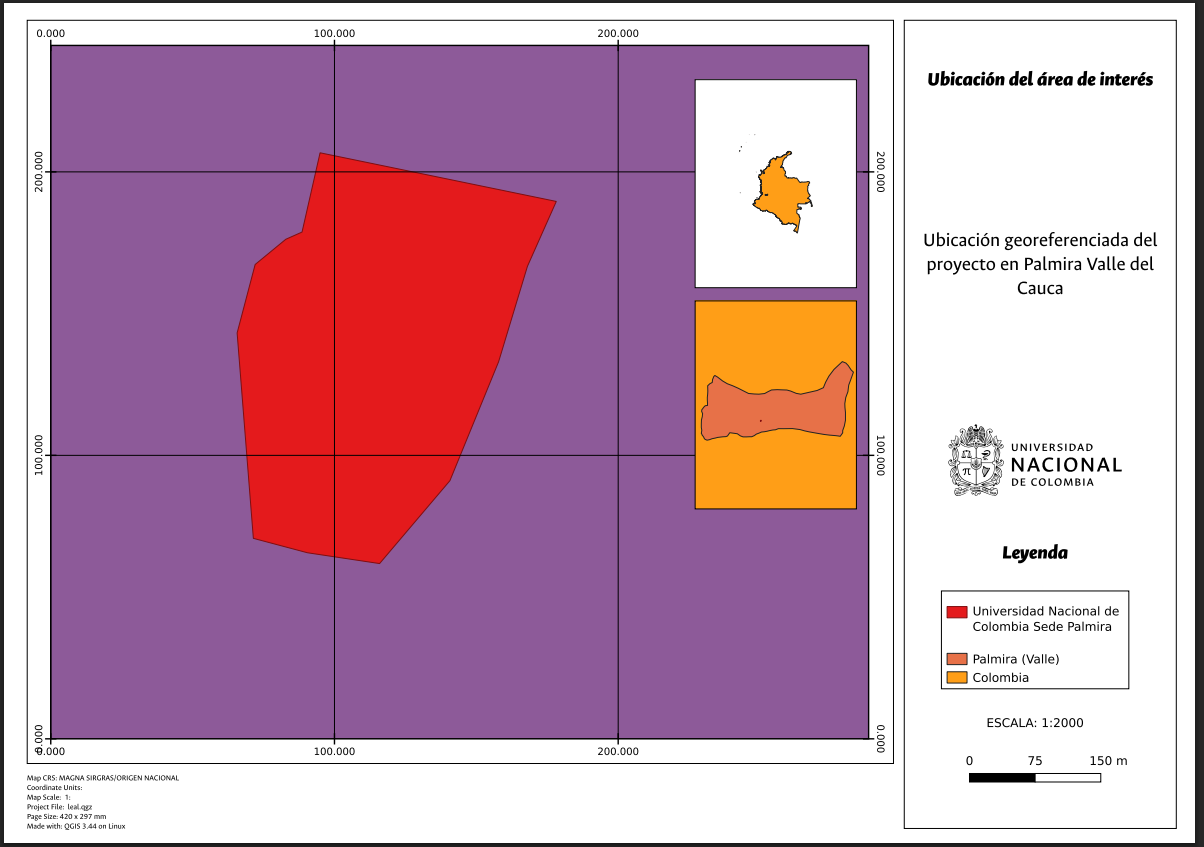
\includegraphics[width=0.9\textwidth]{../tesis/00Figuras/localizacion.png}

        \vspace{0.2cm}
        \footnotesize \textit{Mapa de ubicación georreferenciada del proyecto.}
    \end{columns}
\end{frame}

% =============================================================================
% SECCIÓN 5: APORTE Y ÉTICA (4 min)
% =============================================================================
\section{Aporte y Responsabilidad}

\begin{frame}{De la Estimación Empírica a la Precisión de Datos}
    \begin{columns}[T]
        \column{0.5\textwidth}
        \begin{block}{Tres impactos concretos}
            \begin{enumerate}
                \item \textbf{Factores de emisión:} Evidencia empírica para incorporar BSF en marcos climáticos globales (IPCC Tier 3)
                \item \textbf{Optimización operativa:} Detección temprana de ineficiencias (sobrepoblación, exceso humedad, aireación deficiente)
                \item \textbf{Trazabilidad MRV:} Base para certificación en mercados de carbono (Verra/VCS)
            \end{enumerate}
        \end{block}

        \column{0.5\textwidth}
        \begin{alertblock}{Protocolo de respuesta operativa}
            \begin{itemize}
                \item \textcolor{verdeOK}{\textbf{Verde:}} Emisiones en rango aeróbico. Acumulación de créditos de carbono.
                \item \textcolor{naranjaAlerta}{\textbf{Ámbar:}} Tendencia al alza CO$_2$/O$_2$. Revisar humedad.
                \item \textcolor{rojoAlerta}{\textbf{Rojo:}} Pico de CH$_4$ detectado. Intervención inmediata (volteo).
            \end{itemize}
        \end{alertblock}

        \vspace{0.2cm}
        \centering
        \footnotesize \textit{La predicción como activador de control de procesos.}
    \end{columns}
\end{frame}

\begin{frame}{Compromisos Ético-Epistemológicos}
    \begin{block}{El sistema como herramienta de soporte, no de sustitución}
        La comprensión más robusta emerge de la interacción dialógica entre la señal del sensor y la experiencia empírica del operador.
    \end{block}

    \vspace{0.3cm}
    \centering
    \begin{tikzpicture}[scale=0.9, transform shape,
        comp/.style={rectangle, rounded corners, draw, minimum width=3cm, minimum height=1cm, align=center, font=\small}]

        \node[comp, fill=unalRojo!10] (t1) at (0,2) {Transparencia\\Algorítmica (XAI)};
        \node[comp, fill=unalRojo!10] (t2) at (4,2) {Soberanía\\de Datos};
        \node[comp, fill=unalRojo!10] (t3) at (8,2) {Compatibilidad\\con Saberes};

        \node[comp, fill=gray!10, minimum width=10cm] (base) at (4,0) {Edge Computing + Documentación Abierta + Co-diseño Local};

        \draw[->, thick, >=stealth] (t1) -- (base);
        \draw[->, thick, >=stealth] (t2) -- (base);
        \draw[->, thick, >=stealth] (t3) -- (base);
    \end{tikzpicture}

    \vspace{0.3cm}
    \footnotesize \textit{La tecnología no es neutral. El monitoreo ambiental debe ser instrumento de empoderamiento, no de vigilancia.}
\end{frame}

% =============================================================================
% SECCIÓN 6: CIERRE (3 min)
% =============================================================================
\section{Cierre}

\begin{frame}{Objetivo General y Cronograma}
    \begin{columns}[T]
        \column{0.55\textwidth}
        \begin{alertblock}{Frase para llevar}
            \small
            ``Transformar la bioconversión de una caja negra biológica a un proceso \textbf{transparente}, tecnológicamente \textbf{viable} y verificable \textbf{climáticamente}.''
        \end{alertblock}

        \vspace{0.2cm}
        \textbf{Horizonte:} 42 meses (ago 2023 -- ene 2027)\\
        \textbf{Presupuesto:} 267 MM COP\\
        \textbf{Financiamiento:} Mixto (UNAL + recursos propios)

        \column{0.45\textwidth}
        \centering
        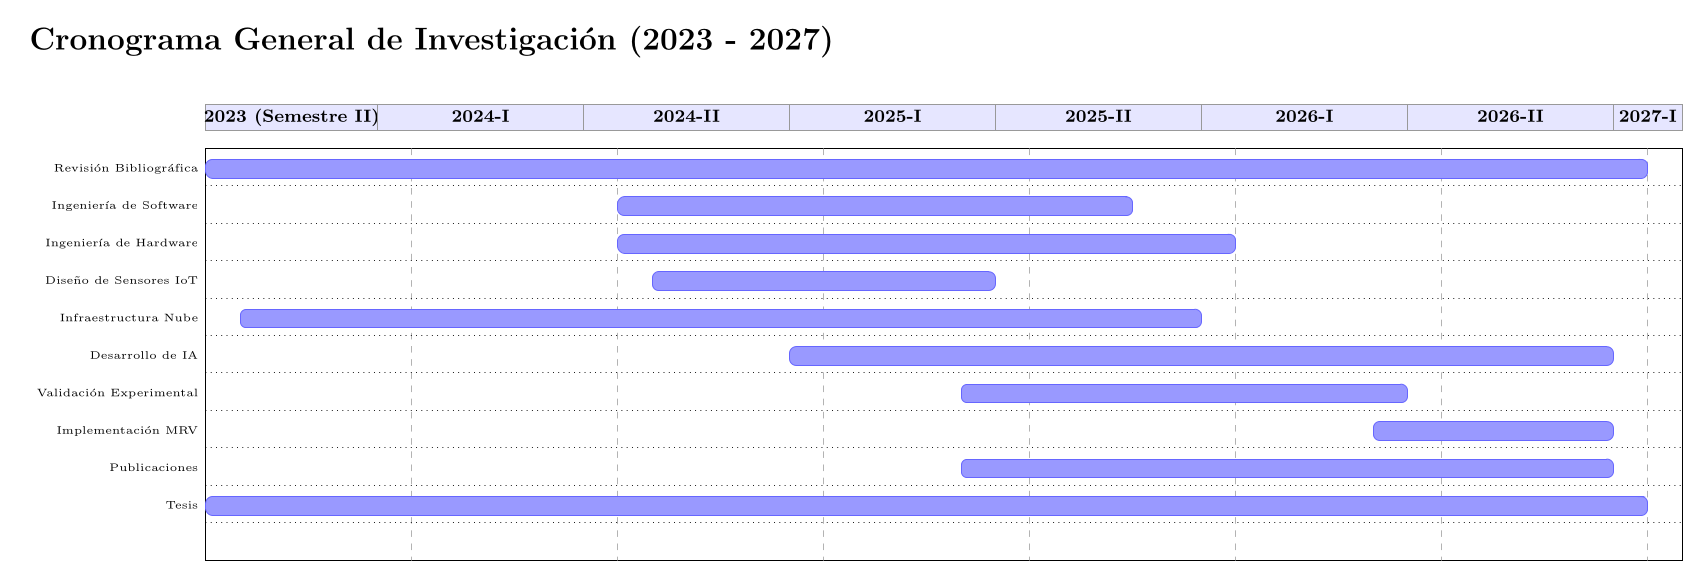
\includegraphics[width=\textwidth]{../tesis/00Figuras/gant.png}

        \vspace{0.2cm}
        \footnotesize \textit{Cronograma de ejecución.}
    \end{columns}
\end{frame}

\begin{frame}{}
    \centering
    \vspace{2cm}
    {\Huge \textbf{Gracias}}

    \vspace{1cm}
    {\large John Jairo Leal Gómez}

    \vspace{0.5cm}
    \texttt{jjlealg@unal.edu.co}

    \vspace{0.3cm}
    \footnotesize Doctorado en Estudios Ambientales\\
    Universidad Nacional de Colombia -- Sede Palmira

    \vspace{1cm}
    
\includegraphics[width=2cm]{../tesis/00Figuras/00f00EscudoUN2016.jpg}
\end{frame}

\end{document}
